% region preamble
% mnras_template.tex 
%
% LaTeX template for creating an MNRAS paper
%
% v3.0 released 14 May 2015
% (version numbers match those of mnras.cls)
%
% Copyright (C) Royal Astronomical Society 2015
% Authors:
% Keith T. Smith (Royal Astronomical Society)

% Change log
%
% v3.0 May 2015
%    Renamed to match the new package name
%    Version number matches mnras.cls
%    A few minor tweaks to wording
% v1.0 September 2013
%    Beta testing only - never publicly released
%    First version: a simple (ish) template for creating an MNRAS paper

%%%%%%%%%%%%%%%%%%%%%%%%%%%%%%%%%%%%%%%%%%%%%%%%%%
% Basic setup. Most papers should leave these options alone.
\documentclass[fleqn,usenatbib]{mnras}

% MNRAS is set in Times font. If you don't have this installed (most LaTeX
% installations will be fine) or prefer the old Computer Modern fonts, comment
% out the following line
% Depending on your LaTeX fonts installation, you might get better results with one of these:
%\usepackage{mathptmx}
%\usepackage{txfonts}

% Use vector fonts, so it zooms properly in on-screen viewing software
% Don't change these lines unless you know what you are doing
\usepackage[T1]{fontenc}

% Allow "Thomas van Noord" and "Simon de Laguarde" and alike to be sorted by "N" and "L" etc. in the bibliography.
% Write the name in the bibliography as "\VAN{Noord}{Van}{van} Noord, Thomas"
\DeclareRobustCommand{\VAN}[3]{#2}
\let\VANthebibliography\thebibliography
\def\thebibliography{\DeclareRobustCommand{\VAN}[3]{##3}\VANthebibliography}


%%%%% AUTHORS - PLACE YOUR OWN PACKAGES HERE %%%%%

% Only include extra packages if you really need them. Common packages are:
\usepackage{graphicx}	% Including figure files
\usepackage{amsmath}	% Advanced maths commands
\usepackage{amssymb}	% Extra maths symbols
\usepackage{newtxtext,newtxmath}

%%%%%%%%%%%%%%%%%%%%%%%%%%%%%%%%%%%%%%%%%%%%%%%%%%

\newcommand{\RCR}{\ensuremath{R_{\textrm{CR}}}}
\newcommand{\Rot}{\ensuremath{\mathcal{R}}}
\newcommand{\Vc}{\ensuremath{V_{\textrm{c}} }}
\newcommand{\PS}{\ensuremath{\Omega_{\textrm{p}}}}
\newcommand{\Rb}{\ensuremath{R_{\textrm{b}}}}

\newcommand{\Nbody}{$N$-body}
\newcommand{\AREPO}{\textsc{AREPO}}
\newcommand{\SMUGGLE}{SMUGGLE}

%%%%% AUTHORS - PLACE YOUR OWN COMMANDS HERE %%%%%

% Please keep new commands to a minimum, and use \newcommand not \def to avoid
% overwriting existing commands. Example:
%\newcommand{\pcm}{\,cm$^{-2}$}	% per cm-squared

% endregion

% region title
%%%%%%%%%%%%%%%%%%% TITLE PAGE %%%%%%%%%%%%%%%%%%%

% Title of the paper, and the short title which is used in the headers.
% Keep the title short and informative.
\title[Stellar Bars and Gas]{Stellar Bars in Isolated Gas-Rich Spiral Galaxies Do Not Slow Down}

\author[A. Beane et al.]{Angus Beane,$^{1}$\thanks{E-mail: angus.beane@cfa.harvard.edu (AB)}
Lars Hernquist,$^{1}$
Elena~D'Onghia,$^{2,3}$
Federico~Marinacci,$^{4}$
Charlie Conroy,$^{1}$
Jia~Qi,$^{5}$\newauthor
Laura~V.~Sales,$^{6}$
Paul~Torrey,$^{5}$
Mark~Vogelsberger$^{7}$
\\
% List of institutions
$^{1}$Center for Astrophysics $|$ Harvard \& Smithsonian,  Cambridge, MA, USA\\
$^{2}$Department of Physics, University of Wisconsin-Madison, Madison, WI, USA\\
$^{3}$Department of Astronomy, University of Wisconsin-Madison, Madison, WI, USA\\
$^{4}$Department of Physics \& Astronomy `Augusto Righi', University of Bologna, Bologna, Italy\\
$^{5}$Department of Astronomy, University of Florida, Gainesville, FL, USA\\
$^{6}$Department of Physics \& Astronomy, University of California, Riverside, CA, USA\\
$^{7}$Department of Physics, Massachusetts Institute of Technology, Cambridge, MA, USA\\
}

% These dates will be filled out by the publisher
\date{Accepted XXX. Received YYY; in original form ZZZ}

% Enter the current year, for the copyright statements etc.
\pubyear{2022}

% endregion

% Don't change these lines
\begin{document}
\label{firstpage}
\pagerange{\pageref{firstpage}--\pageref{lastpage}}
\maketitle

% Abstract of the paper
\begin{abstract}
Elongated bar-like features are ubiquitous in galaxies, occurring at the centers
of approximately two-thirds of spiral disks.  Due to gravitational interactions
between the bar and the other components of galaxies, it is expected that
angular momentum and matter will redistribute over long (Gyr) timescales in
barred galaxies. Previous work ignoring the gas phase of galaxies has
conclusively demonstrated that bars should slow their rotation over time due to
their interaction with dark matter halos. We have performed a simulation of a
Milky Way-like galactic disk hosting a strong bar which includes a
state-of-the-art model of the interstellar medium and a live dark matter halo.
In this simulation the bar pattern does not slow down over time, and instead
remains at a stable, constant rate of rotation. This behavior has been observed
in previous simulations using more simplified models for the interstellar gas
but it has remained unexplained. We propose that the gas phase of the disk and
the dark matter halo act in concert to stabilize the bar pattern speed and
prevent the bar from slowing down or speeding up. We find that in a Milky
Way-like disk, a gas fraction of only about 5\% is necessary for this mechanism
to operate. This result naturally explains why nearly all observed bars rotate
rapidly and is especially relevant for our understanding of how the Milky Way
arrived at its present state.
\end{abstract}

% Select between one and six entries from the list of approved keywords.
% Don't make up new ones.
\begin{keywords}
keyword1 -- keyword2 -- keyword3
\end{keywords}

%%%%%%%%%%%%%%%%%%%%%%%%%%%%%%%%%%%%%%%%%%%%%%%%%%

%%%%%%%%%%%%%%%%% BODY OF PAPER %%%%%%%%%%%%%%%%%%

\section{Introduction}
Elongated bar-like features are ubiquitous in galaxies, occurring at the centers
of approximately two-thirds of spiral disks \citep{2000AJ....119..536E,
2007ApJ...657..790M} and in our own Milky Way \citep{1957AJ.....62...19J,
1991ApJ...379..631B}. The ubiquity of bars is not difficult to explain, since
stellar disks simulated in isolation almost always form bar-like structures
\citep{1971ApJ...168..343H}. Several studies have shown that a spherical
potential, such as from a stellar bulge or dark matter halo, acts to stabilize a
stellar disk against the bar instability \citep{1973ApJ...186..467O,
1976AJ.....81...30H}.

It is more difficult to reconcile numerical simulations with the observed
pattern speeds of extragalactic bars. Currently, the best technique for
measuring the pattern speeds of individual galaxies is the Tremaine-Weinberg
method \citep{1984ApJ...282L...5T, 2011MSAIS..18...23C}. This method has
recently been applied to samples of galaxies from the MaNGA survey
\citep{2019MNRAS.482.1733G, 2020MNRAS.491.3655G}. These recent studies confirm
what was found in earlier studies -- that nearly all extragalactic bars are fast
rotators (i.e., they rotate close to their maximum rotation rate)

This is a problem for theoretical simulations, for which there is ample evidence
that galactic bars should resonantly interact with the dark matter halo, causing
the bar to slow down over time \citep{1992ApJ...400...80H, 2000ApJ...543..704D,
2002MNRAS.330...35A, 2002ApJ...569L..83A, 2003MNRAS.341.1179A,
2003MNRAS.346..251O, 2005MNRAS.363..991H, 2006ApJ...637..214M,
2007MNRAS.375..460W, 2009ApJ...697..293D}. The physical mechanism of this
interaction can be understood as an angular form of dynamical friction between
the bar and the dark matter halo. While studied in detail for the bar
\citep{1984MNRAS.209..729T, 1985MNRAS.213..451W}, this process is generic for
any non-axisymmetric disturbance \citep{1972MNRAS.157....1L}. For an old but
still useful review of bar dynamics, see \citet{1993RPPh...56..173S}

Bar pattern speeds are usually measured using the parameter $\Rot=\RCR/\Rb$,
where \RCR{} is the corotation radius and \Rb{} is the bar length.\footnote{The
radius of corotation \RCR{} is defined for circular orbits as the radius at
which the orbital frequency is equal to the pattern speed, \PS{}, of a given
non-axisymmetric feature. In a galaxy with a constant circular velocity \Vc{},
it is given by $\RCR = \Vc / \PS$.} Galaxies with $\Rot < 1.4$ are considered
``fast rotators'' while galaxies with $\Rot > 1.4$ are considered ``slow
rotators'' \citep{2000ApJ...543..704D}. Galaxies with $\Rot < 1$ are not thought
to be stable \citep{1980AA....81..198C}. Observational estimates of the pattern
speeds of bars indicate that nearly all galaxies have $1 < \Rot <
1.4$ \citep{2011MSAIS..18...23C, 2015AA...576A.102A, 2019MNRAS.482.1733G,
2020MNRAS.491.3655G}.

While the interaction between the bar and a dark matter halo is well-understood
theoretically, this is not the case for the interaction between a bar and a
gaseous disk. Some argue that the gas disk should slow down the bar more, while
others argue that the tendency of the bar to drive gas inwards means the bar
should speed up due to the effect of the gas disk.

In this work, we present a simulation of an isolated, gas-rich disk galaxy. Our
galaxy exhibits some similarities to the Milky Way, described in more detail in
Section XX. Surprisingly, we find that the pattern speed of the bar in this
galaxy is constant with time. We find that with even modest gas fractions of
about 5\%, our isolated galaxy displays no evolution in pattern speed over about
$8\,\textrm{Gyr}$. This behavior has been observed in a few previous works, but
we are the first to exhibit that the behavior ought to be present in a large
fraction of galaxies. We are also the first to provide a physical explanation of
the behavior with clear observational predictions.

In section 2, \dots

% The expectation that a dark matter halo acts to slow down a bar is in conflict
% with observational estimates of bar pattern speeds. Bar rotation rates are
% typically classified by the dimensionless ratio
% % \begin{equation}
% % \Rot = \RCR/R_b\textrm{,}
% % \end{equation}
% where \RCR{} is the radius of corotation and $R_b$ is the length of the
% bar.\footnote{The radius of corotation \RCR{} is defined for circular orbits as
% the radius at which the orbital frequency is equal to the pattern speed,
% $\Omega_p$, of a given non-axisymmetric feature. In a galaxy with a constant
% circular velocity $V_c$, it is given by $\RCR = V_c / \Omega_p$.} Galaxies with
% $\Rot < 1.4$ are considered ``fast rotators'' while galaxies with $\Rot > 1.4$
% are considered ``slow rotators''\cite{2000ApJ...543..704D}. Galaxies with $\Rot
% < 1$ are not thought to be stable\cite{1980AA....81..198C}. Observational
% estimates of the pattern speeds of bars indicate that nearly all galaxies have
% $1 < \Rot < 1.4$\cite{2011MSAIS..18...23C, 2015AA...576A.102A,
% 2019MNRAS.482.1733G, 2020MNRAS.491.3655G}.

% The role of gas on the evolution of the bar is less well-understood. Since the
% gas phase typically only contributes about $10-20\%$ of the mass of a galaxy at
% the present day, one might naively expect it to have a subdominant effect on the
% bar. However, because gas is collisional, it can participate in non-resonant
% angular momentum exchange with the bar\cite{2011MNRAS.415.1027H}. Thus,
% numerical work has shown that the gas phase can have a stronger influence on a
% bar than its contribution to the mass of a galaxy would
% suggest\cite{2010ApJ...719.1470V, 2013MNRAS.429.1949A}.

\section{Methods}

\subsection{Initial Conditions}
The initial setup of the galactic disk used in this work follows closely the
GALAKOS model \citep{2020ApJ...890..117D}, which uses a modified version of the
\texttt{MakeNewDisk} code \citep{2005MNRAS.361..776S}. The GALAKOS model has
three components - a radially exponential and vertically isothermal stellar
disk, and a stellar bulge and dark matter halo following a Hernquist profile
\citep{1990ApJ...356..359H}. All \Nbody{} runs in this work used the same setup
parameters as the GALAKOS disk, more details of which can be found in the
original paper.

The addition of the gas phase was done as follows. The version of
\texttt{MakeNewDisk} used for the original GALAKOS model can generate a gas disk
which is radially exponential and in vertical gravito-hydrodynamic balance. We
modified the radial profile of this code in order to allow us to generate a disk
with a constant surface density within some cut-off radius, and then
exponentially declining beyond that radius with the scale-length of the stellar
disk. Our fiducial model used an initial surface density of
$20\,M_{\odot}/\textrm{pc}^2$ and a cut-off radius of $9.3\,\textrm{kpc}$. The
initial gas disk is generated with a temperature of $10^4\,\textrm{K}$ and solar
metallicity.

After generating the gaseous disk in this way, we stitched the gas disk together
with the GALAKOS \Nbody{} disk (and bulge and dark matter halo) after the
GALAKOS disk has been allowed to evolve for $1.5\,\textrm{Gyr}$. The purpose of
allowing the GALAKOS disk to evolve first for a short period of time is to allow
for the bar to form unimpacted by the presence of the gas. We found that
including the gas before the bar has formed disrupts the formation of the bar,
as has been seen in previous work \citep[e.g.,][]{2013MNRAS.429.1949A}.
Throughout this work, we consider $t=0$ for the \Nbody{} run to be the time at
which we added the gas phase for the SMUGGLE run (i.e., we ignore the first
$1.5\,\textrm{Gyr}$ of evolution of the \Nbody{} disk when the bar is forming).

We made one additional modification when stitching the gas disk together with
the \Nbody{} disk - we created a hole within the central $4\,\textrm{kpc}$. This
hole guards against an initial dramatic infall of gas within the bar region,
which we found to destroy the bar. It is not uncommon for observed barred
galaxies to have gas deficits in the bar region \citep[though not in the very
center;][]{1993RPPh...56..173S}. Therefore, our practice of allowing the gas
distribution to have a hole in the central region is consistent with our choice
to begin the simulations with a bar already formed.

\begin{figure}
\centering
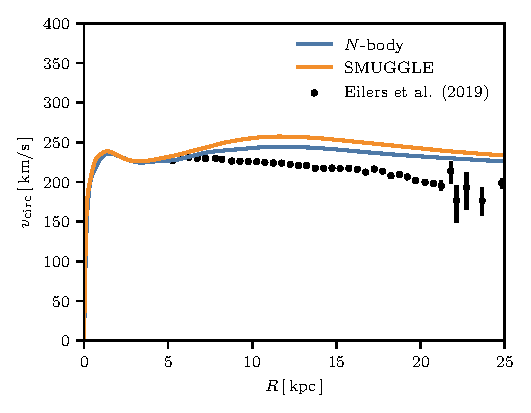
\includegraphics[width=9cm]{fig/vcirc.pdf}
\caption{The circular velocity curve of our initial setups. This
curve is shown for the \Nbody{} run (blue) and the SMUGGLE run (orange)
compared to observational estimates for the Milky
Way \citep{2019ApJ...871..120E}. We see that the circular velocity curve for
both runs is marginally larger than the Milky Way's, but still comparable. The
SMUGGLE circular velocity curve is larger than the \Nbody{} curve due to the
additional mass in the gas phase.}
\label{fig:vcirc}
\end{figure}

We used a mass resolution of $7.5\times10^3\,M_{\odot}$ for the baryonic
components (initial stellar disk, stellar bulge, and gas) and a mass resolution
of $3.75\times10^4\,M_{\odot}$ for the dark matter halo. This mass resolution is
closest to ``level 3'' in the AURIGA simulations \citep{2017MNRAS.467..179G}.
This corresponds to approximately $6.4\times10^6$ particles in the stellar disk,
$1.1\times10^6$ in the bulge, $1.2\times10^6$ in the gas disk, and
$25.3\times10^6$ in the dark matter halo. We used a softening length of
$0.02\,\textrm{kpc}$ for all components. Snapshots were saved at equal intervals
of $0.005$ in the time units of the simulation,
$\textrm{kpc}/(\textrm{km}/\textrm{s})$.

\subsection{Numerical Model}
We use the Stars and MUltiphase Gas in GaLaxiEs (SMUGGLE) model
\citep{2019MNRAS.489.4233M} implemented within the moving-mesh, finite-volume
hydrodynamics and gravity code \AREPO{} \citep{2010MNRAS.401..791S}. The SMUGGLE
model additionally includes radiative heating and cooling, star formation, and
stellar feedback. Explicit gas cooling and heating of the multi-phase
interstellar medium is implemented, covering temperature ranges between $10$ and
$10^8\,\textrm{K}$.

Star formation occurs in cells above a density threshold
($n_{\textrm{th}}=100\,\textrm{cm}^{-3}$) with a star-formation efficiency of
$\epsilon = 0.01$. Star formation converts gas cells into star particles which
represent single stellar populations with a Chabrier initial mass
function \citep{2003PASP..115..763C}. For each star particle, the deposition of
energy, momentum, mass, and metals from stellar winds and supernovae is modeled.
Photo-ionization and radiation pressure are modeled using an approximate
treatment. A more detailed description of this model can be found in the
flagship SMUGGLE paper \citep{2019MNRAS.489.4233M}.

We used the fiducial model parameters, except that we increased the number of
effective neighbors $N_{\textrm{ngb}}$ for the deposition of feedback from
$64$ to $512$. We found that a lower value of $N_{\textrm{ngb}}$ resulted in
inefficient photo-ionization feedback since the photo-ionizing budget had not
been exhausted after deposition into $64$ neighboring cells. We also used an
updated version of SMUGGLE using a new mechanical feedback routine similar to
the one described in \citet{2018MNRAS.480..800H}. This updated routine is a
tensor renormalization which ensures linear and angular momentum conservation
to machine precision.

In addition to the SMUGGLE model, we considered a simpler model of the
interstellar medium based upon \citet{2003MNRAS.339..289S}. In this model, the
multiphase nature of the interstellar medium is modeled in a subgrid manner by
allowing each resolution element to have a ``cold'' and ``hot'' component, with
the equation of state of the gas suitably modified. Gas is allowed to
interchange between the ``cold'' and ``hot'' components through processes such
as cooling and stellar feedback. Cold gas is allowed to undergo star formation.
We refer to this model as the ``smooth interstellar medium'' model, and it is
described in more detail in \citet{2019MNRAS.489.4233M}.

\subsection{Bar Analysis}
The analysis of various bar properties is performed as follows. First, the
pattern speed is measured from the angle of the second Fourier component. We
measured the second Fourier component by computing,
\begin{equation}
\begin{split}
A_2 &= \sum_i m_i e^{i 2 \phi_i} \\
A_0 &= \sum_i m_i \textrm{,}
\end{split}
\end{equation}
where $m_i$ and $\phi_i$ are the mass and azimuthal angle of each particle,
respectively. We computed $A_2$ and $A_0$ in cylindrical bins of width
$0.5\,\textrm{kpc}$ from radii of $0$ to $30\,\textrm{kpc}$. We defined the
angle of the bar $\phi_b$ to be twice the angle of the complex number $A_2$ as
measured in the bin extending from a radius of $2.5$ to $3\,\textrm{kpc}$.
After correcting for the periodicity of $\phi_b$, we measured the pattern
speed as one-half the two-sided finite gradient of $\phi_b$ as a function of
time.

\begin{figure}
\centering
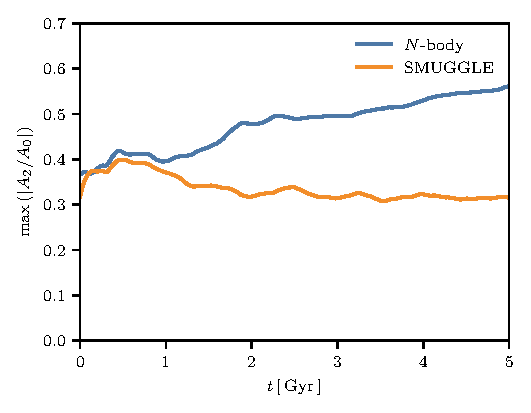
\includegraphics[width=9cm]{fig/A2_over_A0.pdf}
\caption{\textbf{Evolution of bar strength.} The bar strength is measured as
the maximum of the second Fourier component divided by the zeroth Fourier
component. We see that in the
\Nbody{} case (blue) the bar strength increases with time, consistent with
previous results showing that the bar strength increases as bars slow down. In
the SMUGGLE case (orange), we see that the bar strength remains roughly
constant, possibly slightly decreasing with time. This is also consistent with
the expected relation between pattern speed and strength since the bar in this
case is not slowing down.}
\label{fig:strength}
\end{figure}

\begin{figure*}
\centering
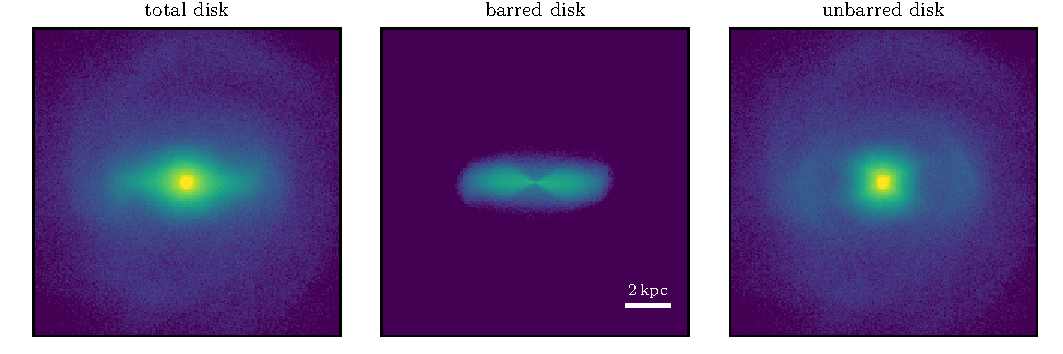
\includegraphics[width=18cm]{fig/bar_decomp.pdf}
\caption{\textbf{Disk decomposition into the barred and unbarred disk.} This
procedure is based on \citet{2016MNRAS.463.1952P} The \textit{left panel} shows
a face-on surface density projection through the stellar component of the
\SMUGGLE{} simulation (disk and bulge) at $t=1\,\textrm{Gyr}$. The
\textit{middle panel} shows the component of the disk identified as being
trapped in the bar while the \textit{right panel} shows the component of the
disk identified as not being trapped in the bar. The fact that the untrapped
stars form a roughly axisymmetric structure indicates our bar decomposition is
sufficiently accurate.}
\label{fig:decomp}
\end{figure*}

The time evolution of the bar strength, defined as the maximum of
$\left|A_2/A_0\right|$ as a function of radius, is shown in Extended Data
Fig.~\ref{fig:strength}. The quantity $\left|A_2/A_0\right|$ varies from $0$
to $1$, with larger values indicating a stronger bar pattern. We see that in
the \Nbody{} case, $\left|A_2/A_0\right|$ increases over time as the bar pattern
slows. This is consistent with previous \Nbody{} simulations which showed a
clear correlation between the bar pattern speed and the bar
strength\cite{2003MNRAS.341.1179A}. In the SMUGGLE case, we see that the bar
strength has an initial drop but then remains at a roughly constant, but
slightly decreasing, strength. This is consistent with the pattern speed in the
SMUGGLE case being roughly constant or slightly increasing.

Computing the length of the bar and the torque on the bar by different
components requires us to decompose the disk into a component which is trapped
by the bar and a component which is untrapped. In order to do this, we follow
closely the technique developed in ref.\cite{2016MNRAS.463.1952P} We analyzed
the orbit of each star particle (meaning initial disk, bulge, and newly formed
stars) by extracting the $x$-$y$ positions of the apoapse of each in a frame
corotating with the bar (apoapses are defined as local maxima in $r$). For
each apoapse, we searched for the $19$ closest apoapses in time and applied a
$k$-means clustering algorithm on this set of $20$ points with $k=2$. We then
computed for each of the two clusters the average angle from the bar
$\left<\Delta \phi\right>_{0,1}$, the standard deviation in $R$ of the points
${\sigma_R}_{0,1}$, and the average radius of the cluster
$\left<R\right>_{0,1}$. At each apoapse, a particle was considered to be in
the bar if it met the following criteria:
\begin{equation}
\textrm{max}\left(\left<\Delta \phi\right>_{0,1}\right) < \pi / 8
\end{equation}
\begin{equation}
\frac{{\sigma_R}_0 + {\sigma_R}_1}{\left<R\right>_0 + \left<R\right>_1} < 0.22
\end{equation}
These criterion are slightly different and simplified from the ones used in
ref.\cite{2016MNRAS.463.1952P}, but we found them to empirically work well at
decomposing the disk into a bar and disk component. In Extended Data
Fig.~\ref{fig:decomp}, we show an example of this decomposition. The
\textit{left} panel shows a surface density projection of the stellar disk and
bulge (including newly formed stars) from the SMUGGLE model after
$1\,\text{Gyr}$ of evolution in a frame such that the bar is aligned with the
$x$-axis. The \textit{middle} panel shows a projection of the subset of stars
that are identified as being trapped in the bar and the \textit{right} panel
shows a projection of the stars that are not identified as being trapped. The
fact that the \textit{right} panel is roughly axisymmetric indicates the bar
decomposition is performing adequately.

After the disk has been decomposed into a trapped and untrapped component, we
measured the bar length as being the radius $R_b$ which encapsulates $99\%$ of
the stars identified as being trapped in the bar, allowing for some outliers.
For the computation of the torque, we used the tree algorithm in
\texttt{MakeNewDisk}\cite{2005MNRAS.361..776S} customized to be accessible
from \texttt{Python} using \texttt{Cython}. This algorithm is based on the
\texttt{TREESPH} code\cite{1989ApJS...70..419H}. We constructed a tree with an opening angle of $0.35$ using
only the star particles identified as being trapped in the bar. We then queried the tree at the locations of all
resolution elements in the other components and computed the torque of the bar
on such components. The torque on the bar by the other components is simply
the negative of the torque on the other components by the bar. A similar
method was applied in measuring the torque for the disk when the pattern speed
is kept constant, as is done in Fig.~\ref{fig:equil}.

% \subsection{Idealized Mock Light Images}
% We created synthetic mock light images at $1024^2$ resolution in
% Fig.~\ref{fig:overview} for the \textit{Hubble Space Telescope} using a
% post-processed Monte Carlo radiation transfer simulation with the SKIRT9 code
% including secondary emission from dust\cite{2020AC....3100381C}. Emission from
% star particles was calculated assuming a Bruzual-Charlot spectral energy
% distribution\cite{2003MNRAS.344.1000B} and a Chabrier initial stellar mass
% function\cite{2003PASP..115..763C}. The luminosity from each star particle was
% smoothed using a cubic spline kernel with each star particle being assigned a
% smoothing length equal to its distance to its $32$nd closest neighbor. We
% launched $10^9$ photon packets per simulation segment. For star particles
% which were present in the initial simulation (i.e., initial disk and bulge
% particles), we assumed that they have an age of $5\,\textrm{Gyr}$ and solar
% metallicity. For star particles in the SMUGGLE simulation which are newly
% formed, we used their recorded ages and metallicities.

% For the SMUGGLE simulations, we included absorption and emission from dust. We
% assumed the THEMIS (The Heterogeneous dust Evolution Model for Interstellar
% Solids) dust model\cite{2017AA...602A..46J} to convert gas metallicity and
% mass density to dust mass density. For the \Nbody{} simulations we ran the
% SKIRT9 code in a mode without an obscuring medium, but otherwise applied the
% same procedure.

% We used the profiles for filters F814W, F606W, and F475W on the Advanced
% Camera for Surveys (ACS) instrument for red, green, and blue pixel values,
% respectively. Filtered fluxes were converted to RGB values using an $\arcsinh$
% scaling following ref.\cite{2004PASP..116..133L} Scalings and cutoff values
% were adjusted manually to create visually appealing images. Filter profiles
% were provided by the Spanish Virtual Observatory Filter
% Service\cite{2012ivoa.rept.1015R, 2020sea..confE.182R}.

\subsection{Plotting Details}
We saved snapshots in intervals of $0.005$ in the time units of the
simulation, $\textrm{kpc}/(\textrm{km}/\textrm{s})$, which is very nearly
equal to $1\,\textrm{Gyr}$ (it is $\sim0.977\,\textrm{Gyr}$). Therefore,
throughout this work we referred to the native code time unit as
$\textrm{Gyr}$. None of our results are sensitive to this choice.

In order to remove numerical noise in several quantities we computed, we
applied a Savitzky-Golay filter \citep{1964AnaCh..36.1627S} as implemented in
\texttt{scipy} using a window length of $81$ and polynomial order of $3$. This
filter was applied to plots of pattern speeds, bar lengths and strengths,
torques, and angle differences.

\section{Discussion}
Our setup is initially out of equilibrium, but we found that after
$\sim500\,\textrm{Myr}$, the entire system has settled into a steady-state
configuration and initial transients appear not to affect the results after
this point. The constant surface density of the initial gas disk is important
for ensuring the gas disk is dense enough in order for comparisons to real
galaxies to be appropriate.

We computed the circular velocity curve of our model using the \texttt{AGAMA}
package\cite{2019MNRAS.482.1525V}. We fit the baryonic component (stellar
disk, bulge, gas, and newly formed stars) with an axisymmetric cylindrical
spline with $20$ grid points in both the radial and vertical direction
spanning $0.2$ to $50\,\textrm{kpc}$ in the radial direction and from $0.02$
to $10\,\textrm{kpc}$ in the vertical direction. We fit the dark matter halo
using a spherically symmetric multipole fit with a maximum angular harmonic
coefficient of $l=2$. We plot the circular velocity curve in Extended Data
Fig.~\ref{fig:vcirc} compared to observational
estimates\cite{2019ApJ...871..120E}. The SMUGGLE disk (which includes
additional mass in the form of gas) has a slightly higher circular velocity
than the \Nbody{} disk which, itself, is slightly higher than the
observational estimates.

\begin{figure}
    \centering
    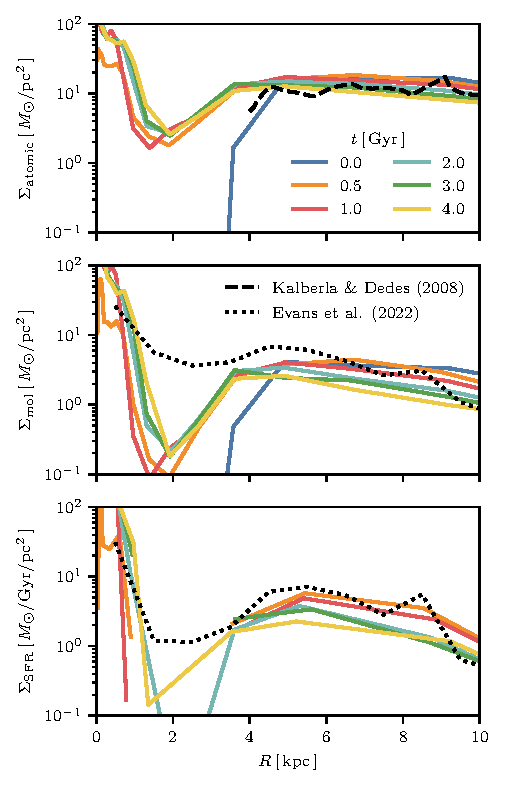
\includegraphics[width=9cm]{fig/surf_dens.pdf}
    \caption{The time evolution of the atomic gas surface density
    (\textit{upper}), molecular gas surface density (\textit{middle}) and the
    star formation rate (SFR) surface density (\textit{lower}) at various times
    during our fiducial simulation. Colored lines indicate the profiles at
    selected times during the simulation while the black dashed lines indicate
    observations for the atomic gas \citep{2008AA...487..951K} and black dotted
    lines indicate a model which allows the CO-to-H$_2$ conversion factor
    $X_{\textrm{CO}}$ to vary with metallicity \citep{2022ApJ...929L..18E}.
    Molecular gas surface densities were provided separately (N. Evans, private
    communication). We see that the molecular gas and SFR surface densities are
    within an order of magnitude of the Milky Way's typical values at all times.
    We see a sharp decrease in the gas and SFR surface densities along the
    extent of the bar from $\sim1$ to $\sim4\,\textrm{kpc}$, related to the gas
    inflow in this region.}
    \label{fig:surf}
\end{figure}

We also show the evolution of the surface density profile in Extended Data
Fig.~\ref{fig:surf} We find that in our simulation the atomic and molecular
gas surface density and the SFR surface density is broadly consistent with the
expected values for the Milky
Way\cite{2008AA...487..951K,2022ApJ...929L..18E}. The discrepancy between $1$
and $4\,\textrm{kpc}$ in the molecular and SFR surface density is likely due
to the fact that the distances to molecular clouds which underlines this work
used a simple kinematic distance based on an axisymmetric model of the Milky
Way\cite{2017ApJ...834...57M}, which is not accurate in the bar region where
gas has large non-circular velocities.

The pattern speed evolution of this setup is given in Extended Data
Fig.~\ref{fig:GFM}, which shows that the pattern speed evolves in a similar
manner to the SMUGGLE case shown in Fig.~\ref{fig:prop}.


% \subsection{Figures and tables}

% Figures and tables should be placed at logical positions in the text. Don't
% worry about the exact layout, which will be handled by the publishers.

% Figures are referred to as e.g. Fig.~\ref{fig:example_figure}, and tables as
% e.g. Table~\ref{tab:example_table}.

% % Example figure
% \begin{figure}
% 	% To include a figure from a file named example.*
% 	% Allowable file formats are eps or ps if compiling using latex
% 	% or pdf, png, jpg if compiling using pdflatex
% 	\includegraphics[width=\columnwidth]{example}
%     \caption{This is an example figure. Captions appear below each figure.
% 	Give enough detail for the reader to understand what they're looking at,
% 	but leave detailed discussion to the main body of the text.}
%     \label{fig:example_figure}
% \end{figure}

% % Example table
% \begin{table}
% 	\centering
% 	\caption{This is an example table. Captions appear above each table.
% 	Remember to define the quantities, symbols and units used.}
% 	\label{tab:example_table}
% 	\begin{tabular}{lccr} % four columns, alignment for each
% 		\hline
% 		A & B & C & D\\
% 		\hline
% 		1 & 2 & 3 & 4\\
% 		2 & 4 & 6 & 8\\
% 		3 & 5 & 7 & 9\\
% 		\hline
% 	\end{tabular}
% \end{table}


\section{Conclusions}

The last numbered section should briefly summarise what has been done, and describe
the final conclusions which the authors draw from their work.

\section*{Acknowledgements}

The Acknowledgements section is not numbered. Here you can thank helpful
colleagues, acknowledge funding agencies, telescopes and facilities used etc.
Try to keep it short.

%%%%%%%%%%%%%%%%%%%%%%%%%%%%%%%%%%%%%%%%%%%%%%%%%%
\section*{Data Availability}

 
The inclusion of a Data Availability Statement is a requirement for articles published in MNRAS. Data Availability Statements provide a standardised format for readers to understand the availability of data underlying the research results described in the article. The statement may refer to original data generated in the course of the study or to third-party data analysed in the article. The statement should describe and provide means of access, where possible, by linking to the data or providing the required accession numbers for the relevant databases or DOIs.




%%%%%%%%%%%%%%%%%%%% REFERENCES %%%%%%%%%%%%%%%%%%

% The best way to enter references is to use BibTeX:

\bibliographystyle{mnras}
\bibliography{ref} % if your bibtex file is called example.bib


% Alternatively you could enter them by hand, like this:
% This method is tedious and prone to error if you have lots of references
%\begin{thebibliography}{99}
%\bibitem[\protect\citeauthoryear{Author}{2012}]{Author2012}
%Author A.~N., 2013, Journal of Improbable Astronomy, 1, 1
%\bibitem[\protect\citeauthoryear{Others}{2013}]{Others2013}
%Others S., 2012, Journal of Interesting Stuff, 17, 198
%\end{thebibliography}

%%%%%%%%%%%%%%%%%%%%%%%%%%%%%%%%%%%%%%%%%%%%%%%%%%

%%%%%%%%%%%%%%%%% APPENDICES %%%%%%%%%%%%%%%%%%%%%

\appendix

\section{Some extra material}

If you want to present additional material which would interrupt the flow of the main paper,
it can be placed in an Appendix which appears after the list of references.

%%%%%%%%%%%%%%%%%%%%%%%%%%%%%%%%%%%%%%%%%%%%%%%%%%


% Don't change these lines
\bsp	% typesetting comment
\label{lastpage}
\end{document}

% End of mnras_template.tex
